\documentclass[serif,mathserif,final]{beamer}
\mode<presentation>{\usetheme{Lankton}}


\setbeamertemplate{caption}[numbered] % number figs
\usepackage[
  orientation=landscape,
  size=custom,
  width=152.400,height=91.400,%size=a0, % paper size
  scale=1.3 % font scale factor
  ]{beamerposter}


% Graphics Path
\usepackage{graphicx}
\graphicspath{{"../figs/"}}

% OTHER PACKAGE CALLS
\usepackage[utf8]{inputenc}
\usepackage{amsmath,amssymb,physics} % math symbols
\usepackage{siunitx}
\sisetup{round-mode = figures, round-precision = 3}
\usepackage{tikz}
\usetikzlibrary{
	shapes,
    arrows,
    shapes.geometric,
    positioning,
}

% Define block styles
\tikzstyle{object} = [
	rectangle,
    draw,
    fill=blue!20,
    text width=2.5cm,
    text badly centered,
    rounded corners]

\tikzstyle{action} = [
	rectangle,
	draw,
    text width=4.5cm,
    text centered,
    rounded corners]

\tikzstyle{arrow} = [draw, -latex']
\tikzstyle{noarrow} = [draw, dashed]

% set consistent font size
%\tikzset{every picture/.style={font issue=\footnotesize},
%         font issue/.style={execute at begin picture={#1\selectfont}}
%         }


% eg and ie
\usepackage{xspace}
\newcommand*{\eg}{e.g.\@\xspace}
\newcommand*{\ie}{i.e.\@\xspace}

% this package loads last except for biblatex
\usepackage{cleveref}

% Use BibLaTeX
\usepackage[
	backend=biber,
	doi=false,
	url=false,
	isbn=false,
	maxnames=3,
	minnames = 1,
	style=numeric-comp,
	sorting=none,
	natbib=true,
	firstinits=true,
	isbn=false
  ]{biblatex}
\renewbibmacro{in:}{}
\addbibresource{../library.bib}
\AtEveryBibitem{
  \clearfield{month}
  \clearlist {language}
  \clearfield{pages}
  \clearfield{pages}
  \clearfield{volume}
  \clearfield{number}
  \clearfield{title}
}
\setbeamertemplate{bibliography item}[text] % don't print the silly symbols

%-- Header and footer information ----------------------------------
\newcommand{\footleft}{\url{water.columbia.edu}}
\newcommand{\footright}{\url{james.doss-gollin@columbia.edu}}
\title{Global-Local Interactions Modulate Tropical Moisture Export to the Ohio River Basin}
\author{James Doss-Gollin\inst{1,2} \quad David Farnham\inst{1,2} \quad Upmanu Lall\inst{1,2}}
\institute
{\inst{1} Columbia Water Center \quad \inst{2} Department of Earth and Environmental Engineering, Columbia University}

%-------------------------------------------------------------------


%-- Main Document --------------------------------------------------
\begin{document}

% Statistical Macros
\def\ci{\perp\!\!\!\perp}
\def\ex{\mathbb{E}}
\def\prob{\mathbb{P}}
\def\ind{\mathbb{I}}
\def\grad{\triangledown}
\def\bigo{\mathcal{O}}
\def\normal{\mathcal{N}}
\def\bern{\text{Bernoulli}}
\def\logit{\text{logit}}
\def\binom{\text{Bin}}
\def\poiss{\text{Poiss}}
\def\cauchy{\text{Cauchy}}
\def\sigmoid{\vb{\sigma}}
\def\given{\big|}
\def\stan{\texttt{Stan~}}

%A little bit on why this region is interesting & our broad hypotheses (floods come from a hierarchy of causal mechanisms)
%Establish that synoptic features modulate moisture flux -- I think this is already done with the maps that I have of flux given cyclone positions
%Establish that "global" features (i.e. PNA, AMO) modulate these synoptic features -- again I think plots of cyclone tracks given different PNA phases is good
%Explain that the purpose of the Bayesian model is to learn how the large-scale features modulate the local features
%Present the model very briefly
%Finish by taking a subset of the data, predicting using the observed values of PNA + AMO, and comparing to just regressing on PNA & AMO with no intermediate step.
\begin{frame}{}
  \begin{columns}[t]

    %-- Column 1 ---------------------------------------------------
    \begin{column}{0.2\linewidth}

        \begin{block}{Conceptual Framework}
    Making credible forecasts of future flood probabilities from sub-seasonal to decadal timescales \cite{Merz2014} requires understanding the cross-timescale dynamics that regulate the joint distribution of the frequency, intensity, and persistence of rainfall.
    Case study \cite[\ie][]{Grams2014} and theory support the view that persistent intense rainfall does not occur randomly, but rather that the large-scale transport \& convergence of moisture is governed by specific circulations mechanisms which are in turn modulated by global-scale circulations and persistent, low-frequency boundary conditions.

    For example, the April 2011 flooding in the Ohio-Mississippi river system led to sever damage.
    As \cref{fig:apr2011} shows, the monthly rainfall was driven by a strong and persistent jet which steered multiple cyclones along highly similar trajectories.
    \begin{figure}
        \begin{tikzpicture}[node distance = 1.cm, auto, font=\sffamily]
	% Place nodes
	\node [action] (boundary) {Boundary Forcings\\ (\ie ENSO)};
	\node [object, below= of boundary] (circulation) {Circulation Anomaly\\ (\ie PNA)};
	\node [object, below=of circulation] (steering) {Moisture Steering\\ (\ie Cyclone)};
	\node [action, below= of steering] (flood) {High Flood Potential};
	% Draw edges
	\path [arrow] (boundary) -- (circulation);
    \path [arrow] (circulation) -- (steering);
    \path [arrow] (steering) -- (flood);
\end{tikzpicture}
~\hfill
        \includegraphics[width=0.6\columnwidth]{flooding_2011_flooding}
        \caption{(L) Mechanistic casual hierarchy for extreme, regional floods. (R) Tracked cyclones (lines) and monthly-mean \SI{250}{\hecto\pascal} winds for April 2011.}
        \label{fig:apr2011}
    \end{figure}
\end{block}

        \begin{block}{Research Questions \& Data Used}
    \begin{enumerate}
        \item What synoptic weather patterns lead to intense moisture transport into the Ohio River Basin?
        \item How do planetary-scale circulations modulate these synoptic weather patterns?
        \item What are the conditional probabilities of moisture transport into the region, given synoptic and planetary circulation indices?
        \item How can predictions of low-frequency modes of planetary circulation inform risk of extreme, regional flooding?
    \end{enumerate}
    We use the Ohio River Basin (\cref{fig:study-area}) to anchor a case study, focusing on the DJF season during which the well-known 1937 flood occurred.
    We use 6-hourly reanalysis data from ERA-Interim \cite{Dee2011} (1979-2015) and cyclone tracks generated by Donna Lee \cite{Booth2015} using the TRACK algorithm \cite{Hodges1994}.
\end{block}



    \end{column}%1

    %-- Column 2 ---------------------------------------------------
    \begin{column}{0.18\linewidth}
        \begin{block}{Study Area \& Variable Definitions}
    \begin{figure}
        \centering
        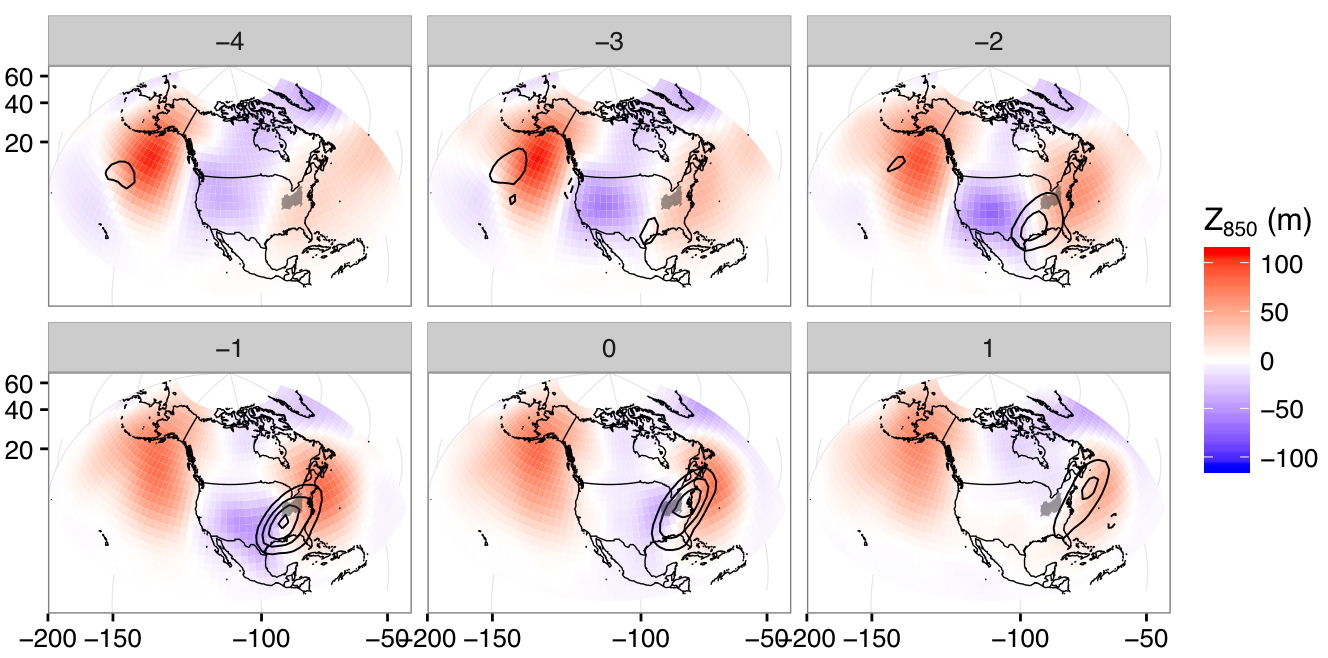
\includegraphics[width=0.95\columnwidth]{../FigExternal/djf_composites}
        \caption{Composite anomalies of \SI{500}{\hecto\pascal} geopotential height (color) and precipitable water (contours) from 4 days preceding 113 regional intense precipitation days in the Ohio River Basin to one day following. Regional intense precipitation days defined as at least 10\% of GHCN rain gauges exceeding 99th percentile. From \cite{Farnham2016}.}
        \label{fig:djf-composites}
    \end{figure}
    Study of regional intense precipitation events in the Ohio River Basin (\cref{fig:djf-composites}) reveals the importance of a ridge (somtimes stationary, sometimes transient) over the Western Atlantic and a transient cyclone propagating eastward.
    To study this, we define the following variables, separated into planetary-scale and synoptic-scale:
    \begin{description}
        \item[Moisture] the daily net moisture flux into Ohio River Basin region (\cref{fig:study-area}, green box)
        \item[Planetary] 30-day moving average of the PNA and NAO indices from the CPC
        \item[Synoptic] Mean daily SST anomalies over the Gulf of Mexico (\cref{fig:study-area}, blue); and the \SI{850}{\hecto\pascal} the geopotential height anomalies over the West Atlantic (purple) and the Eastern United States (red).
    \end{description}
    The Eastern U.S. low and Western Atlantic high capture the geopotential height gradient over the region, representing dynamical drivers (see \cite{Farnham2016} for details), and the SST anomalies over the moisture source region \cite[see][and references therein]{Steinschneider2016a} represent thermodynamic drivers.
    \begin{figure}
        \centering
        \includegraphics[width=0.85\columnwidth]{map_inset}
        \caption{Study Area. Shaded area shows the Ohio River Basin. Boxes show locations of indices described above.}
        \label{fig:study-area}
    \end{figure}
\end{block}


    \end{column}%2

    %-- Column 3 ---------------------------------------------------
    \begin{column}{0.18\linewidth}
        \begin{block}{Synoptic Modulation of Moisture Flux}
    The location of extratropical cyclones modulates moisture flux into the Ohio River Basin.
    To see this, for each time step we take the cyclone closest to the region and assign it to the observed moisture flux for that time step.
    \Cref{fig:track-given-flux} (L) shows the results of a local regression \cite{Loader1999} fit to observed data.
    The statistical model allows us to assign a score from zero to one for the (rescaled) expected moisture flux into the region, given an arbitrary cyclone location.

    The right hand figure further demonstrates that cyclone tracks associated with extremely high flux follow highly similar trajectories.
    \emph{The similarity of these trajectories suggests planetary-scale, steering mechanisms.}
    These tracks also resemble those shown in \cref{fig:apr2011} that led to flooding in April 2011.
    Other factors beyond cyclone position, including GMX temperature and the Western Atlantic Ridge (\cref{fig:study-area}), are included in our statistical model but are not plotted.
    \begin{figure}
        \includegraphics[width=0.45\columnwidth]{locfit_weight_predicted_observed}~
        \includegraphics[width=0.5\columnwidth]{moisture_cyclone_tracks_given_flux}
        \caption{(L) Expected moisture transport given cyclone location. Units are normalized from zero to one. Colors show observation and contours show the statistical model.
                (R) Tracks of extratropical cyclones associated with (L) 70 random DJF days, and (R) the 70 days with highest DJF moisture transport. The ``Moisture'' box of \cref{fig:study-area} is shown for reference.}
        \label{fig:track-given-flux}
    \end{figure}
\end{block}

        \begin{block}{Global-Scale Modulation}

    \begin{figure}
        \includegraphics[width=\columnwidth]{pna_cyclone_map_plot}
        \caption{Cyclone tracks given (L) PNA in negative tercile; (C) neutral PNA; (R) positive PNA}
        \label{fig:track-given-pna}
    \end{figure}
\end{block}


    \end{column}%3

    %-- Column 4 ---------------------------------------------------
    \begin{column}{0.2\linewidth}

      \begin{block}{Bayesian Conditional Probability Estimation}
    To estimate the conditional probabilities of moisture flux conditional on synoptic features, and of synoptic features conditional on planetary-scale features, we build a Bayesian model which allows for simultaneous parameter estimation.
    This model takes requires three fundamental data blocks:
    \begin{enumerate}
        \item $y_{N \times 1}$, the observed data (in this case, the moisture flux)
        \item $X_{N \times p}$, the ``local'' factors that directly govern the $y$
        \item $Z_{N \times k}$, the ``global'' factors that are hypothesized to govern the $X$
    \end{enumerate}
    Then, the model is formulated as
    \begin{align}
        y_t & \sim \normal \qty(\beta_0 + X'_t \beta, \sigma^2) \quad t = 1, \ldots, T \label{eq:yX}\\
        X_{t,j} &\sim \normal \qty(\alpha_{0,j} + Z'_t \alpha_j, \tau_j^2) \quad j = 1, \ldots, p \label{eq:XZ}
    \end{align}
    To estimate the parameters $\beta_0, \beta, \sigma, \alpha_0, \alpha, \tau$ we use Hamiltonian Monte Carlo Markov Chain sampling using the Bayesian programming language Stan \cite{Carpenter2016}.
    Because of the large amount of data available, we apply noninformative priors \cite{Gelman2014}.

\end{block}

      \begin{block}{Model Inferences}
    \begin{figure}
        \centering
        \includegraphics[width=0.95\columnwidth]{bayesian_posterior}
        \caption{\num{4000} draws from posterior distribution specified by \cref{eq:yX,eq:XZ}.}
        \label{fig:posterior}
    \end{figure}
    Interpreting the results of \cref{fig:posterior} requires noting the ordering of the $X$ and $Z$ variables; for example, \texttt{alpha[1,3]} gives the coefficient of $Z_{1}$ (PNA) on $X_3$ (GMX SSTs).
    In the first (local-moisture) step, we note that the effect of the dynamical $X$ variables (the low and high height anomalies; $\beta_1, \beta_2$) is far greater than the effect of the thermodynamic variable (the GMX SSTs; $\beta_3$).
    This comparison is valid because all $X$ and $Z$ have been standardized.
    Other variables should be explored before drawing more general conclusions.
    It is also of note that the magnitude of the effect of increasing the W. Atlantic High ($\beta_1$) is somewhat larger than increasing the magnigude of the Eastern U.S. Low $(\beta_2)$.
    In the second (global-local) step, we see that a positive PNA provides feedbacks that both support and inhibit moisture flux to the Ohio River Basin, suppressing the high and GMX SSTs ($\alpha_{1,1}, \alpha_{1,3}$) but enhancing the low ($\alpha_{1,2}$) in the positive phase.
    The NAO also provides both moisture-inhibiting and moisture-enhancing effects ($\alpha_{2,1:3}$).
\end{block}


    \end{column}%3


    %-- Column 5 ---------------------------------------------------
    \begin{column}{0.18\linewidth}
        \begin{block}{Summary of Findings}
    \begin{enumerate}
        \item A finite set of specific synoptic circulation patterns accounts for most DJF moisture transport into the Ohio River Basin
        \item Persistent steering mechanisms such as the PNA and NAO alter the dominant directions of cyclone propagation over the region, leading to changes in moisture transport
        \item The PNA and NAO provide both positive and negative feedbacks on moisture transport to the Ohio River Basin. Modeling these intermediate feedbacks explicity \textbf{improves model propagation of opposing feedbacks and variance} as compared to modeling moisture transport directly on the global-scale indices.
    \end{enumerate}
\end{block}

        \begin{block}{Next Steps \& Discussion}
    \begin{itemize}
        \item Posterior checking (not shown) reveals that modeling all interactions as normal (\cref{eq:yX,eq:XZ}) is an overly strong assumption; specific distributions for specific interactions will address this step
        \item Including additional parameters will reduce model variance
        \item Consideration of GMX SST anomalies as a local feature addresses thermodynamic impact on moisture availability, but is not independent of large-scale circulations; likely not a one-directional causality
        \item Model dependence of global features explicity using copulas \cite[\ie][]{Genest2007}
    \end{itemize}
\end{block}

        \begin{block}{Acknowledgements}
    Thanks to Donna Lee for sharing cyclone tracks.
    Thanks to Yochanan Kushnir, Jimmy Booth, Scott Steinschneider, Pierre Gentine, Casey Brown, Linda Mearns, Katherine Schlef, Melissa Bukovsky, Rachel McCrary, and Seth McGinnis for insightful conversations.
    This project is funded by the Department of Defense Strategic Environmental Research and Development Program (SERDP) grant \# 15 RC02-060.
\end{block}

        \begin{block}{References}
            \renewcommand*{\bibfont}{\footnotesize}
            \printbibliography[heading=none]
        \end{block}


    \end{column}%1

  \end{columns}
\end{frame}
\end{document}
